% !TEX root = ../../thesis.tex

\section{Design Principles} \label{designPrinciples}

In order to address the problems mentioned in the \nameref{problemStatement} (\ref{problemStatement}) section, we adopted and implemented the following design principles.

\subsection{No foreign code execution}

There is no foolproof way of entirely securing a piece of software; even the most mature platforms and operating systems sometimes end up vulnerable to security exploits. However, without the ability to execute code on a platform, it is not directly possible to take advantage of vulnerabilities, even when there is one. Furthermore, the nature of Intertext allowed us to adopt disallowing code execution as a design principle. Intertext clients only accept UIUDL code, which is in XML and is not executable. Should a server send anything else, Intertext clients will simply ignore it. Thus, we can guarantee security for the users, regardless of the platform they are using the Intertext client on.

\subsection{Transparency}

Privacy is a common concern among users; primarily due to the recent scandals and data leaks, people started getting more conscious about their data. There is an increasing demand for users to be more in control and be aware of what is exposed and what is not. In order to address this burning need, we adopted transparency as a design principle. 

The most prominent way of achieving this is to have Intertext clients be in control of all interactions with the device and with external sources and keep logs in order to make them transparent to the user. The above-mentioned principle that no foreign code will be executed goes hand-in-hand in achieving this, as it would be unrealistic to expect complete control as it would be a non-deterministic approach. A good analogy would be to think of Intertext clients as an API endpoint that runs on users devices and exposes fundamental interactions with the host device and external networks through an API in a fully controlled manner. An application could "instruct" the Intertext client via IUIDL to perform some actions, such as making a network request, storing data, and accessing the local storage. Intertext client will then block this action until the user grant permission and keep logs every time before performing an action (Fig \ref{fig:permission_flow})

\begin{figure}
  \centering
  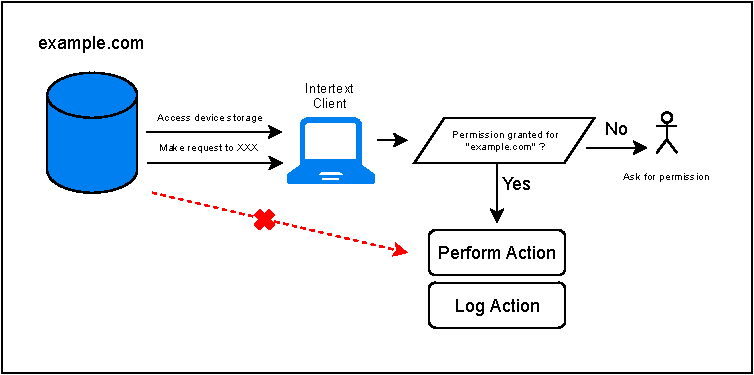
\includegraphics[width=9.2cm]{thesis/paper/images/permission.pdf}
  \caption{A diagram showing the permission flow}%
  \label{fig:permission_flow}%
\end{figure}


\subsection{Component-based approach}

Intertext provides a set of basic components for developers to use build their applications with. In principle, 


\subsection{One language, }


% - design principles
%   - no foreign code executions / only data
%   - no foreign styling / customisable styles
%   - transparency
%     - all front-end ops goes through intertext client (requests from the server)
%     - all requests goes through intertext client (youtube embed etc.)
%   - all platforms shares the same syntax
  
